\documentclass[border=1pt]{standalone}
\usepackage[usenames,dvipsnames]{xcolor}
\usepackage{tikz,array,comment}
\usepackage{tikz-qtree}
\usepackage{sansmath}
\usetikzlibrary{arrows,shapes,automata,patterns,trees,decorations}

\renewcommand{\familydefault}{\sfdefault}
\sffamily\sansmath

\begin{document}

% Set the overall layout of the tree
\tikzset{level 1/.style={level distance=10.0cm}}
\tikzset{level 2+/.style={level distance=1.6cm}}
\tikzset{edge from parent/.append style={->,line width=1.2,shorten >=2.5pt,shorten <=2.5pt}}
% Define styles for leafs
\tikzset{every leaf node/.style={draw,text width=1.09cm,inner sep=2pt,minimum height=0.4cm,align=center}}

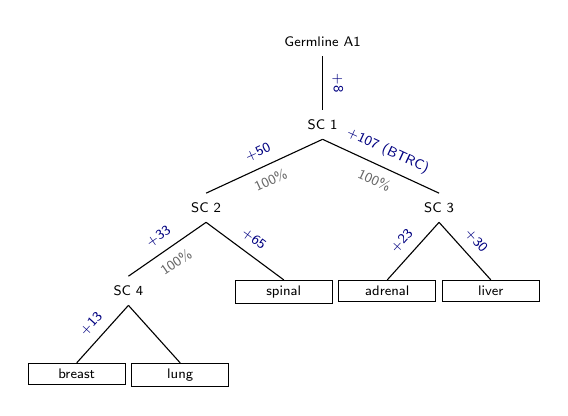
\begin{tikzpicture}[sloped,font=\sansmath\sffamily\normalsize]

\Tree [.\tiny{Germline~A1}
	\edge node[above, NavyBlue]{\tiny{+8}};
 	% Acquired mutations (8): -, -, -, INPP5A, INVS, LGALS13, SLIT1, TNFSF8
	% Acquired mutations (8): 10__134354633__X>Y, 10__98963266__X>Y, 19__44778597__X>Y, 6__131730938__X>Y, 6__50519104__X>Y, 9__101950362__X>Y, 9__105825009__X>Y, 9__116716911__X>Y
	% Acquired mutations (8): 24,55,80,200,201,209,284,305
	% VAF of acquired mutations: mean 25.26%; median 25.09%
	[.\tiny{SC~1} 
		\edge node[above, NavyBlue]{\tiny{+50}} node[below, black!60]{\tiny{100\%}};
 		% Acquired mutations (50): -, -, -, -, -, -, -, -, -, -, -, -, ADK, ARHGAP18, ASCC3, ASTN2, CUZD1, DLG2, ENSG00000186882, ENSG00000209555, ENSG00000219755, ENSG00000220243, ENSG00000221809, ERP44, FAM184A, FKTN, GABBR2, GFRA1, GNA12, GNA14, GPR63, GRID1, HS3ST4, KPNA5, LOC100131500, LOC100132919, LOC729076, OR10W1, PCDH15, PRCP, PRLHR, PRUNE2, RAB23, SEH1L, SHC3, STX11, SUPT5H, TCERG1L, ZNF536, ZNF83
		% Acquired mutations (50): 10__117941181__X>Y, 10__120345140__X>Y, 10__124594542__X>Y, 10__132896117__X>Y, 10__30169005__X>Y, 10__43989381__X>Y, 10__56960415__X>Y, 10__57955358__X>Y, 10__67259978__X>Y, 10__75747164__X>Y, 10__87785576__X>Y, 11__57818048__X>Y, 11__82237372__X>Y, 11__83660465__X>Y, 12__126933980__X>Y, 16__26054565__X>Y, 16__5214155__X>Y, 16__5851742__X>Y, 16__7733510__X>Y, 16__8001212__X>Y, 18__12905622__X>Y, 18__15045444__X>Y, 19__35552353__X>Y, 19__36351696__X>Y, 19__44652253__X>Y, 19__57897877__X>Y, 6__100130338__X>Y, 6__101334520__X>Y, 6__103034674__X>Y, 6__103810336__X>Y, 6__117127430__X>Y, 6__119480716__X>Y, 6__130021483__X>Y, 6__141812628__X>Y, 6__144496653__X>Y, 6__50534952__X>Y, 6__57180847__X>Y, 6__97417052__X>Y, 7__2798617__X>Y, 9__100276456__X>Y, 9__101815469__X>Y, 9__107431799__X>Y, 9__108142026__X>Y, 9__118892426__X>Y, 9__119966859__X>Y, 9__78648387__X>Y, 9__78768991__X>Y, 9__79451567__X>Y, 9__88816952__X>Y, 9__90860126__X>Y
		% Acquired mutations (50): 11,15,30,44,48,58,66,74,83,86,91,97,107,115,116,118,135,138,145,153,168,170,174,182,185,186,188,189,190,191,192,193,195,206,216,219,231,252,259,266,268,269,271,280,281,289,290,292,322,328
		% VAF of acquired mutations: mean 19.11%; median 18.98%
		[.\tiny{SC~2} 
			\edge node[above, NavyBlue]{\tiny{+33}} node[below, black!60]{\tiny{100\%}};
 			% Acquired mutations (33): -, -, -, -, -, -, -, -, -, -, -, -, -, A1CF, AMAC1L1, APBA2, ATRNL1, COL13A1, DLG2, ENSG00000201938, ENSG00000217870, ENSG00000219293, ENSG00000222436, EPC1, LOC389787, LOC644489, NELL1, ROS1, SLC35F1, SORCS1, TMEM132D, TMEM132D, ZNF649
			% Acquired mutations (33): 10__108403050__X>Y, 10__110054257__X>Y, 10__110710074__X>Y, 10__117497577__X>Y, 10__130230535__X>Y, 10__32654300__X>Y, 10__33920504__X>Y, 10__33978032__X>Y, 10__52263467__X>Y, 10__57689541__X>Y, 10__57944469__X>Y, 10__66422894__X>Y, 10__71255829__X>Y, 11__21127304__X>Y, 11__40432908__X>Y, 11__83658548__X>Y, 12__126730170__X>Y, 12__128113143__X>Y, 12__128845242__X>Y, 15__24276991__X>Y, 15__27129009__X>Y, 18__11582759__X>Y, 18__4110314__X>Y, 19__57034973__X>Y, 6__117752227__X>Y, 6__118310721__X>Y, 6__50568504__X>Y, 6__99144022__X>Y, 9__102564991__X>Y, 9__105790749__X>Y, 9__119906713__X>Y, 9__77620839__X>Y, 9__97892203__X>Y
			% Acquired mutations (33): 4,6,29,40,46,50,62,67,71,73,90,93,99,100,109,114,121,132,140,149,161,167,175,181,223,225,245,275,283,288,299,302,326
			% VAF of acquired mutations: mean 18.22%; median 18.32%
			[.\tiny{SC~4} 
				\edge node[above, NavyBlue]{\tiny{+13}};
 				% Acquired mutations (13): -, -, -, C9orf5, CDH23, ENPP3, ENSG00000213742, FAM182B, LOC100129633, LOC100134139, PARD3, TFAP2B, TMEM132C
				% Acquired mutations (13): 10__110512707__X>Y, 10__34419015__X>Y, 10__73230224__X>Y, 11__23740966__X>Y, 11__40628227__X>Y, 12__127741648__X>Y, 16__34450096__X>Y, 16__9643678__X>Y, 20__25706058__X>Y, 6__132075413__X>Y, 6__50909762__X>Y, 9__110925162__X>Y, 9__116561273__X>Y
				% Acquired mutations (13): 1,54,69,126,128,144,157,184,213,221,256,293,296
				% VAF of acquired mutations: mean 20.38%; median 19.76%
				\node[black,draw,text width=1.09cm,inner sep=2pt,align=center]{\tiny breast};  
				% Present mutations: 104; Reported mutations: 210 
				\edge node[above, NavyBlue]{};
 				\node[black,draw,text width=1.09cm,inner sep=2pt,align=center]{\tiny lung};  
				% Present mutations: 91; Reported mutations: 96 
			]
			\edge node[above, NavyBlue]{\tiny{+65}};
 			% Acquired mutations (65): -, -, -, -, -, -, -, -, -, -, -, -, -, -, -, -, A2BP1, A2BP1, A2BP1, ANKRD30B, ANXA2P3, ATAD1, ATP10A, CLEC16A, CNNM1, COL28A1, DEFB112, DLG2, DLG2, ENSG00000200079, ENSG00000201196, ENSG00000217870, ENSG00000217894, ENSG00000222452, ENSG00000222512, FLJ34223, KCNK18, KIAA1279, KLHL32, LILRB3, LOC100132919, LOC340268, MACROD2, MACROD2, MAN1A1, MED29, NLP, NXPH1, NXPH1, OCA2, PARD3, PCDH15, RNF20, SAR1A, SDK1, TJP1, TMEM132D, TMEM132D, TMEM132D, TMEM132D, TRDN, TRIM14, UTRN, ZNF528, ZNF568
			% Acquired mutations (65): 10__101107797__X>Y, 10__109260503__X>Y, 10__110011608__X>Y, 10__110505831__X>Y, 10__118904382__X>Y, 10__128306852__X>Y, 10__130217114__X>Y, 10__34419041__X>Y, 10__54329123__X>Y, 10__56286085__X>Y, 10__66289693__X>Y, 10__70445764__X>Y, 10__71632452__X>Y, 10__89525467__X>Y, 11__21612687__X>Y, 11__23115916__X>Y, 11__83285209__X>Y, 11__83652317__X>Y, 12__126853896__X>Y, 12__128268516__X>Y, 12__128550411__X>Y, 12__128642204__X>Y, 12__128680715__X>Y, 15__23664750__X>Y, 15__25783910__X>Y, 15__27787091__X>Y, 16__11075432__X>Y, 16__17888791__X>Y, 16__5818404__X>Y, 16__5881592__X>Y, 16__5903125__X>Y, 16__6329002__X>Y, 16__6836550__X>Y, 16__7318796__X>Y, 18__10177961__X>Y, 18__14740390__X>Y, 19__36621094__X>Y, 19__39059284__X>Y, 19__42129322__X>Y, 19__44578501__X>Y, 19__57610720__X>Y, 19__59464954__X>Y, 20__14276029__X>Y, 20__14809183__X>Y, 20__25429155__X>Y, 6__102992907__X>Y, 6__104027186__X>Y, 6__119610996__X>Y, 6__124021182__X>Y, 6__144924303__X>Y, 6__49276467__X>Y, 6__50173697__X>Y, 6__51288265__X>Y, 6__97473303__X>Y, 7__3768336__X>Y, 7__7439179__X>Y, 7__8478845__X>Y, 7__8765760__X>Y, 7__9812796__X>Y, 9__103356303__X>Y, 9__105709515__X>Y, 9__110136656__X>Y, 9__79928379__X>Y, 9__83267462__X>Y, 9__99878405__X>Y
			% Acquired mutations (65): 7,13,14,21,25,26,35,41,42,52,53,57,63,75,79,81,102,105,106,111,112,119,120,130,131,133,137,139,141,147,148,162,163,176,177,187,202,203,205,210,220,222,235,239,240,241,246,249,250,251,255,257,273,276,277,294,297,301,303,304,306,308,312,321,325
			% VAF of acquired mutations: mean 19.03%; median 18.92%
			\node[black,draw,text width=1.09cm,inner sep=2pt,align=center]{\tiny spinal};  
			% Present mutations: 123; Reported mutations: 120 
		]
		\edge node[above, NavyBlue]{\tiny{+107 (BTRC)}} node[below, black!60]{\tiny{100\%}};
 		% Acquired mutations (107): -, -, -, -, -, -, -, -, -, -, -, -, -, -, -, -, -, -, -, -, -, -, -, -, -, -, -, -, -, -, -, -, -, -, A2BP1, A2BP1, A2BP1, ANXA2P3, ASTN2, BTRC, C10orf129, C20orf191, CASC2, CEP192, CTNNA3, DBC1, DYRK1B, ENSG00000206323, ENSG00000210066, ENSG00000212316, ENSG00000214604, ENSG00000214788, ENSG00000217120, ENSG00000218583, ENSG00000218777, ENSG00000220184, ENSG00000221481, ENSG00000222979, ENSG00000222979, ENSG00000223167, FAM13C, GRID1, HS3ST4, ICK, INA, INCENP, LAMA2, LOC100128304, LOC100129329, LOC100132843, LOC644489, LOC646360, LOC653895, LOC727842, LOC728027, LOC728050, LOC729901, LRRC4C, MACROD2, MACROD2, NLRP8, NRG3, PCDH15, PCDH15, PLCE1, POP4, PPRC1, RAB12, RIMBP2, SEC23IP, SLC16A12, SMG1, SNORD116-19, TLE1, TMEM132D, TRPM3, TTMA, USP7, XYLT1, XYLT1, XYLT1, ZNF30, ZNF415, ZNF420, ZNF536, ZNF536, ZNF677
		% Acquired mutations (107): 10__103185549__X>Y, 10__103851083__X>Y, 10__105029604__X>Y, 10__109684059__X>Y, 10__111440844__X>Y, 10__119809535__X>Y, 10__121672136__X>Y, 10__123142748__X>Y, 10__123176990__X>Y, 10__129930864__X>Y, 10__129995611__X>Y, 10__130355724__X>Y, 10__131089946__X>Y, 10__36464896__X>Y, 10__37680767__X>Y, 10__52157626__X>Y, 10__56698159__X>Y, 10__57030481__X>Y, 10__58639860__X>Y, 10__58963125__X>Y, 10__59261669__X>Y, 10__60728325__X>Y, 10__62934765__X>Y, 10__66289971__X>Y, 10__67522524__X>Y, 10__84237719__X>Y, 10__85037579__X>Y, 10__85385165__X>Y, 10__86683874__X>Y, 10__87497692__X>Y, 10__91253403__X>Y, 10__95991906__X>Y, 10__96954888__X>Y, 11__40229086__X>Y, 11__40993183__X>Y, 11__41006427__X>Y, 11__41306602__X>Y, 11__59495943__X>Y, 11__61666104__X>Y, 11__81008903__X>Y, 11__81013414__X>Y, 11__81013867__X>Y, 12__126641560__X>Y, 12__126845541__X>Y, 12__127279792__X>Y, 12__128358480__X>Y, 12__129547396__X>Y, 12__130583256__X>Y, 15__22871365__X>Y, 15__27411102__X>Y, 16__13038906__X>Y, 16__17118848__X>Y, 16__17168566__X>Y, 16__17454144__X>Y, 16__17828151__X>Y, 16__18760365__X>Y, 16__20150769__X>Y, 16__22560185__X>Y, 16__25573603__X>Y, 16__26519321__X>Y, 16__5973467__X>Y, 16__6748701__X>Y, 16__7330884__X>Y, 16__8206373__X>Y, 16__8384449__X>Y, 16__8956415__X>Y, 18__1101401__X>Y, 18__13079146__X>Y, 18__14844752__X>Y, 18__2114715__X>Y, 18__5862587__X>Y, 18__8554742__X>Y, 19__34750995__X>Y, 19__35400145__X>Y, 19__35618611__X>Y, 19__35635072__X>Y, 19__36821124__X>Y, 19__40094764__X>Y, 19__42312834__X>Y, 19__44991316__X>Y, 19__46786035__X>Y, 19__58326020__X>Y, 19__58483172__X>Y, 19__61142880__X>Y, 20__14463421__X>Y, 20__14833014__X>Y, 20__26062570__X>Y, 6__103399899__X>Y, 6__103477515__X>Y, 6__103604780__X>Y, 6__119817960__X>Y, 6__122215854__X>Y, 6__129508904__X>Y, 6__142312187__X>Y, 6__53035144__X>Y, 6__55918529__X>Y, 6__58602457__X>Y, 6__96859305__X>Y, 6__98144517__X>Y, 6__99123934__X>Y, 9__117468997__X>Y, 9__118381668__X>Y, 9__121221226__X>Y, 9__72590416__X>Y, 9__76957621__X>Y, 9__82200493__X>Y, 9__83417270__X>Y
		% Acquired mutations (107): 0,3,8,9,10,12,16,17,18,19,20,28,31,32,34,36,37,38,39,43,45,47,51,59,60,68,72,78,82,84,87,92,95,96,101,103,104,113,117,122,123,125,127,129,134,136,143,151,154,155,158,159,160,164,165,169,172,178,179,180,183,194,196,197,198,199,208,211,212,218,224,226,227,228,229,230,233,234,236,237,247,248,258,262,263,264,265,270,272,279,282,286,287,295,298,309,310,311,315,316,317,318,319,320,323,324,327
		% VAF of acquired mutations: mean 28.40%; median 23.62%
		[.\tiny{SC~3} 
			\edge node[above, NavyBlue]{\tiny{+23}};
 			% Acquired mutations (23): -, -, -, -, -, -, -, DLGAP1, ENSG00000197911, ENSG00000202438, ENSG00000221175, LOC100131774, MIRN122, MIRN520F, PALM2-AKAP2, PARD3, PCDH15, ROR2, SDK1, SLIT1, SVIL, VPS13A, WNT8B
			% Acquired mutations (23): 10__102226253__X>Y, 10__29461916__X>Y, 10__29919312__X>Y, 10__34647328__X>Y, 10__56493989__X>Y, 10__84904764__X>Y, 10__92437193__X>Y, 10__98841741__X>Y, 11__21728969__X>Y, 11__41595795__X>Y, 15__24014359__X>Y, 18__3602475__X>Y, 18__54242870__X>Y, 19__58850716__X>Y, 6__130937388__X>Y, 6__132319804__X>Y, 6__145323291__X>Y, 6__48902663__X>Y, 6__50179508__X>Y, 7__3882114__X>Y, 9__111851665__X>Y, 9__79055566__X>Y, 9__93339819__X>Y
			% Acquired mutations (23): 2,5,27,49,61,76,94,142,146,150,171,217,242,243,253,254,261,274,278,285,291,313,314
			% VAF of acquired mutations: mean 22.31%; median 22.06%
			\node[black,draw,text width=1.09cm,inner sep=2pt,align=center]{\tiny adrenal};  
			% Present mutations: 138; Reported mutations: 138 
			\edge node[above, NavyBlue]{\tiny{+30}};
 			% Acquired mutations (30): -, -, -, -, -, -, -, -, -, -, -, -, AHCYL1, ANKRD1, C16orf58, ENSG00000206857, ENSG00000212626, ENSG00000219154, ENSG00000221796, KIR3DX1, LAMA1, LOC100129901, LOC100130696, LOC729340, MACROD2, NEDD4L, PCDH15, PRKCB, TMEM132D, TRDN
			% Acquired mutations (30): 10__110299526__X>Y, 10__110441149__X>Y, 10__120608275__X>Y, 10__55990127__X>Y, 10__58187546__X>Y, 10__66554900__X>Y, 10__84909021__X>Y, 10__92678250__X>Y, 10__97714894__X>Y, 12__127478127__X>Y, 12__127553074__X>Y, 12__128320409__X>Y, 12__129034081__X>Y, 16__24089332__X>Y, 16__31462404__X>Y, 18__52907898__X>Y, 18__54062878__X>Y, 18__7066925__X>Y, 18__7340525__X>Y, 19__59741948__X>Y, 1__110359957__X>Y, 20__14753799__X>Y, 6__120890851__X>Y, 6__121308670__X>Y, 6__123538582__X>Y, 6__145591500__X>Y, 6__145717562__X>Y, 6__97912586__X>Y, 7__9237639__X>Y, 9__87569416__X>Y
			% Acquired mutations (30): 22,23,33,56,64,65,70,77,85,88,89,98,108,110,124,152,156,166,173,204,207,214,215,232,238,244,260,267,300,307
			% VAF of acquired mutations: mean 21.73%; median 22.36%
			\node[black,draw,text width=1.09cm,inner sep=2pt,align=center]{\tiny liver};  
			% Present mutations: 145; Reported mutations: 145 
		]
	]
]

\end{tikzpicture}
% \caption{Phylogenetic tree illustrating the evolutionary history of the cancer. The derivation of an evolutionarily-compatible maximum likelihood tree identified 39 putative false-positives or false-negatives (out of 1645; 2.4%). Putative false-positives 36, put. false-negatives 3, put. false neg.-unknowns 3. }
\end{document}
